% Copyright 2004 by Till Tantau <tantau@users.sourceforge.net>.
%
% In principle, this file can be redistributed and/or modified under
% the terms of the GNU Public License, version 2.
%
% However, this file is supposed to be a template to be modified
% for your own needs. For this reason, if you use this file as a
% template and not specifically distribute it as part of a another
% package/program, I grant the extra permission to freely copy and
% modify this file as you see fit and even to delete this copyright
% notice. 

\documentclass{beamer}
\usepackage[utf8]{inputenc}
\usepackage[brazilian]{babel}

% There are many different themes available for Beamer. A comprehensive
% list with examples is given here:
% http://deic.uab.es/~iblanes/beamer_gallery/index_by_theme.html
% You can uncomment the themes below if you would like to use a different
% one:
%\usetheme{AnnArbor}
%\usetheme{Antibes}
%\usetheme{Bergen}
%\usetheme{Berkeley}
%\usetheme{Berlin}
%\usetheme{Boadilla}
%\usetheme{boxes}
\usetheme{CambridgeUS}
%\usetheme{Copenhagen}
%\usetheme{Darmstadt}
%\usetheme{default}
%\usetheme{Frankfurt}
%\usetheme{Goettingen}
%\usetheme{Hannover}
%\usetheme{Ilmenau}
%\usetheme{JuanLesPins}
%\usetheme{Luebeck}
%\usetheme{Madrid}
%\usetheme{Malmoe}
%\usetheme{Marburg}
%\usetheme{Montpellier}
%\usetheme{PaloAlto}
%\usetheme{Pittsburgh}
%\usetheme{Rochester}
%\usetheme{Singapore}
%\usetheme{Szeged}
%\usetheme{Warsaw}

\title{Aula 3 - Unix}

% A subtitle is optional and this may be deleted
\subtitle{Curso de Unix}

\author{PET Computa\c{c}ão}
% - Give the names in the same order as the appear in the paper.
% - Use the \inst{?} command only if the authors have different
%   affiliation.

\institute[UFSC] % (optional, but mostly needed)
{
%
  Departamento de Informática e Estatística\\
  Universidade de Santa Catarina}
% - Use the \inst command only if there are several affiliations.
% - Keep it simple, no one is interested in your street address.

\date{PET Computa\c{c}ão, 2015}
% - Either use conference name or its abbreviation.
% - Not really informative to the audience, more for people (including
%   yourself) who are reading the slides online

\subject{Curso de Unix}
% This is only inserted into the PDF information catalog. Can be left
% out. 

% If you have a file called "university-logo-filename.xxx", where xxx
% is a graphic format that can be processed by latex or pdflatex,
% resp., then you can add a logo as follows:

% \pgfdeclareimage[height=0.5cm]{university-logo}{university-logo-filename}
% \logo{\pgfuseimage{university-logo}}

% Delete this, if you do not want the table of contents to pop up at
% the beginning of each subsection:
\AtBeginSubsection[]
{
  \begin{frame}<beamer>{Sumário}
    \tableofcontents[currentsection,currentsubsection]
  \end{frame}
}

% Let's get started
\begin{document}

\begin{frame}
  \titlepage
\end{frame}

\begin{frame}{Sumário}
  \tableofcontents
  % You might wish to add the option [pausesections]
\end{frame}

% Section and subsections will appear in the presentation overview
% and table of contents.
\section{Redirecionamentos}

\subsection{Redirecionando saída}

\begin{frame}{Redirecionando saída}{$|$ (pipe)}
  \begin{itemize}
  \item { \textbf{Pipe} é um recurso integrado ao terminal que permite redirecionar a saída de um comando para  a entrada de outro.
    }\end{itemize}
          \begin{figure}[h!]
        \centering
        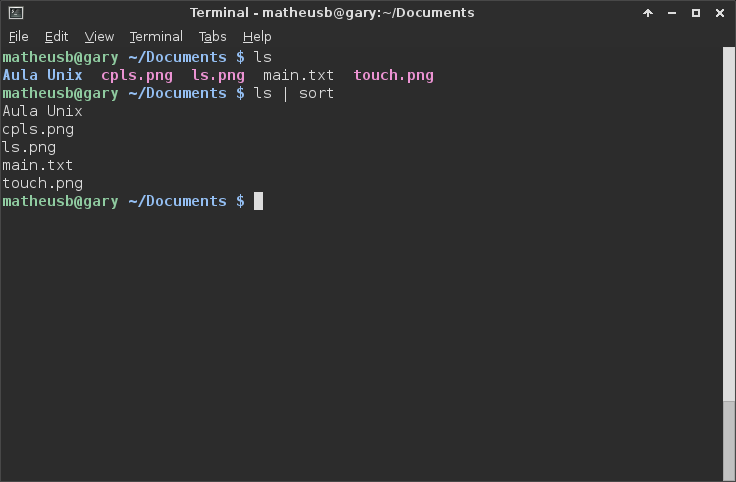
\includegraphics[scale=0.30]{pipe.png}
        \caption{Comando $|$ pipe}
        \label{fig:Comando |}
    \end{figure}
\end{frame}

\begin{frame}{Redirecionando saída}{$>$}
  \begin{itemize}
  \item { O comando \textbf{$>$} redireciona a saida de um comando para um arquivo.
    }\end{itemize}
          \begin{figure}[h!]
        \centering
        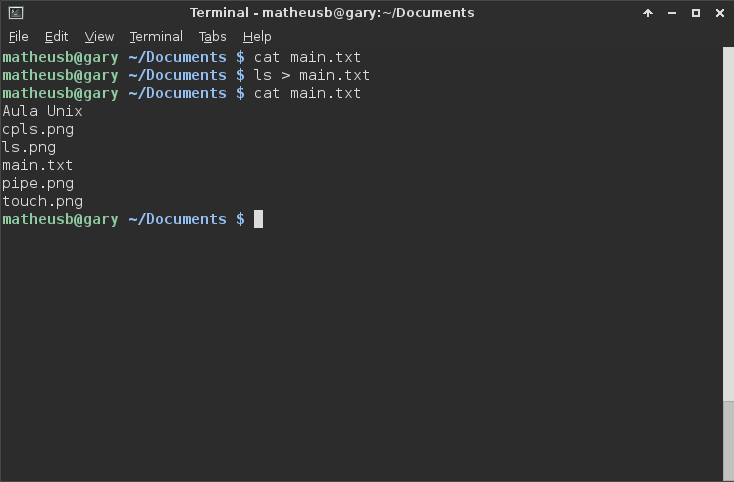
\includegraphics[scale=0.30]{redirecting.png}
        \caption{Comando $>$}
        \label{fig:Comando >}
    \end{figure}
\end{frame}

\begin{frame}{Redirecionando saída}{$>>$}
  \begin{itemize}
  \item { O comando \textbf{$>>$} redireciona a saida de um comando para um arquivo mas diferentemente de \textbf{$>$} ele acrescenta a saida ao arquivo e não substitui o que já existe lá.
    }\end{itemize}
          \begin{figure}[h!]
        \centering
        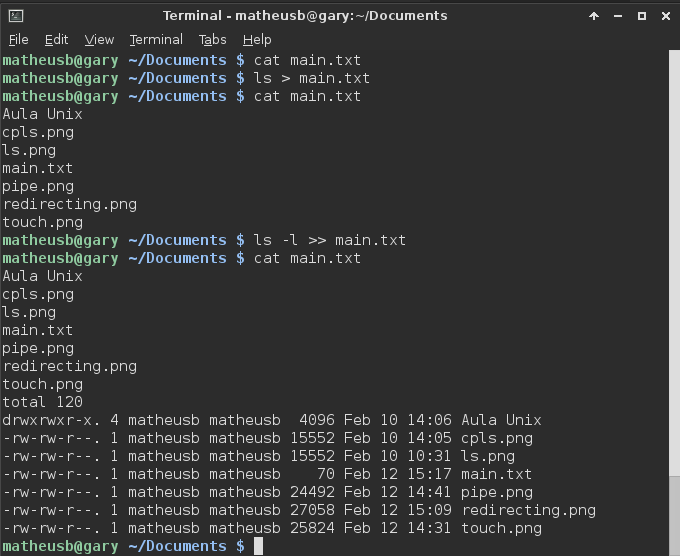
\includegraphics[scale=0.22]{append.png}
        \caption{Comando $>>$}
        \label{fig:Comando >>}
    \end{figure}
\end{frame}

\begin{frame}{Redirecionando saída}{$<$}
  \begin{itemize}
  \item { O comando $<$ redireciona o que há em um arquivo para a entrada de um comando.
    }\end{itemize}
          \begin{figure}[h!]
        \centering
        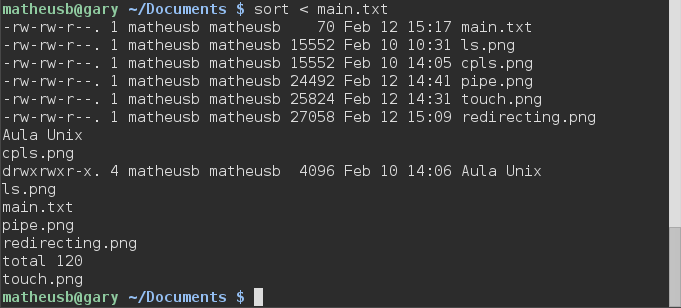
\includegraphics[scale=0.3]{directing.png}
        \caption{Comando $<$}
        \label{fig:Comando <}
    \end{figure}
\end{frame}

\subsection{less}
\begin{frame}{Exibir página}{less}
  \begin{itemize}
  \item {
   O comando less exibe somente uma pagina do arquivo indicado na tela.
    } 
    \item{ \textbf{less arquivo1}, exibe a primeira página do arquivo1.}
    \item{Apertando espaço você passa de página
  }
  \end{itemize}
\end{frame}

\subsection{head}
\begin{frame}{Exibir inicio}{head}
  \begin{itemize}
  \item {
O comando head exibe as 10 primeiras linhas de um arquivo indicado
} 
    \item{ \textbf{head arquivo1} exibe as 10 primeiras linhas do arquivo}
    \item{Para exibir menos linhas usa-se a tag -n, onde n é o número de linhas a menos que 10 que deseja exibir.
  }
 
  \end{itemize}
\end{frame}


\subsection{tail}
\begin{frame}{Exibir fim}{tail}
  \begin{itemize}
  \item {   O comando tail exibe as 10 ultimas linhas do arquivo indicado.
   } 
    \item{ \textbf{tail arquivo1} exibe as 10 ultimas linhas do arquivo1
    }
    \item{Para exibir mais linhas usa-se -n onde n é o número de linhas a mais que você deseja exibir.
  }
  \end{itemize}
\end{frame}

\subsection{grep}
\begin{frame}{Busca no arquivo}{grep}
  \begin{itemize}
  \item {  O comando grep é utilizado para buscar palavras especificas no arquivo.
   } 
    \item{ \textbf{grep} \textit{\textit{item} \textbf{arquivo1} busca a palavra item no arquivo1.
    }}
    \begin{block}{Case sensitive}
O comando grep é case sensitive, ou seja, buscar \textit{Laranja}, \textit{laranja} ou \textit{LARANJA} trará retornos diferentes.
\end{block}
  \end{itemize}
\end{frame}
% You can reveal the parts of a slide one at a time
% with the \pause command:

\section*{Sumário dos comandos}

\begin{frame}{Sumário dos comandos}
\begin{center}
 \begin{tabular}{||c | p{9cm}||} 
 \hline
 \textbf{Comando} & \textbf{Descri\c{c}ão}\\ [0.5ex] 
 \hline\hline
 \vert & Redireciona a saída de um comando para outro\\ 
 \hline
 \hline
 $>$ & Redireciona a saída de um comando para um arquivo\\
 \hline
 $>>$ & Acrescenta a saída de um comando para um arquivo\\
 \hline
 $<$ & Redireciona o que há em um arquivo para a entrada de um comando\\
 \hline
 less & Exibe a primeira página do arquivo desejado\\
 \hline
 head & Mostra as 10 primeiras linhas do arquivo desejado, usa-se a flag -n para mostrar menos do que 10 linhas onde n é o número de linhas desejado\\
 \hline
 tail & Mostra as 10 últimas linhas do arquivo desejado, pode ser utilizado também com a flag -n\\
 \hline
 grep & Pesquisa no arquivo desejado a palavra dada\\
 \hline
\end{tabular}
\end{center}
\end{frame}

\end{document}


